\documentclass{article}

%----------------------------------------
% Packages
%----------------------------------------
\usepackage[left=1in, right=1in, top=1in, bottom=1in]{geometry}
\usepackage{graphicx}
\usepackage{amsmath,amsbsy,amssymb,amsfonts,amsthm}
\usepackage{nicefrac}
\usepackage{mathtools}
\usepackage{color}
\usepackage{xspace} % Correct macro spacing
\usepackage[numbers]{natbib} % For citations
\usepackage{times}
\usepackage{graphicx,subfigure}
%\usepackage[small,bf]{caption}
\usepackage{algorithm,algorithmic}
\usepackage{hyperref}
\usepackage[algo2e]{algorithm2e}

\usepackage{xcolor}
\usepackage{shadethm}

\usepackage{tikz}

\usepackage{fancyhdr}
\pagestyle{fancy}
\lhead{This is my name}
\rhead{this is page \thepage}

\usepackage{fancyhdr}
\pagestyle{fancy}
\lhead{IFT 6085 - Theoretical principles for deep learning}
\rhead{Lecture 19: April 15, 2020}


\newshadetheorem{thm}{Theorem}
\newshadetheorem{defn}[thm]{Definition}
\newshadetheorem{assm}[thm]{Assumption}
\newshadetheorem{prop}[thm]{Property}
\newshadetheorem{eg}[thm]{Example}


\definecolor{shadethmcolor}{HTML}{F0F0F0}
%\definecolor{shadethmcolor}{HTML}{EDEDED}
%\definecolor{shadethmcolor}{HTML}{EDF8FF}
%\definecolor{shaderulecolor}{HTML}{EDF8FF}
%\definecolor{shaderulecolor}{HTML}{45CFFF}
\setlength{\shadeboxrule}{.4pt}


\setlength\parindent{0pt}

% Packages hyperref and algorithmic misbehave sometimes.  We can fix
% this with the following command.
\newcommand{\theHalgorithm}{\arabic{algorithm}}

%----------------------------------------
% Standard macros
%----------------------------------------


%----------------------------------------
% Project-specific macros
%----------------------------------------

%----------------------------------------
% Header
%----------------------------------------
\title{IFT 6085 - Lecture 19 \\ 
Basic results on reinforcement learning}
\date{}

%----------------------------------------
% Document
%----------------------------------------
\begin{document} 

%----------------------------------------
% Abstract
%----------------------------------------
\maketitle

\vspace{-0.5in}
\begin{center}
This version of the notes has not yet been thoroughly checked.
Please report any bugs to the scribes or instructor.
\end{center}
\vspace{0.2in}

\textbf{Scribes}\hfill
\textbf{Instructor:}  Ioannis Mitliagkas\\
\textbf{Winter 2019:} Eugene Vorontsov \& Charles Guille-Escuret\\
\textbf{Winter 2020:} Emre Onur Kahya\\


%----------------------------------------
% Body
%----------------------------------------

\newcommand{\infgc}{\inf_{g \in \mathcal{C}}}
\newcommand{\supgc}{\sup_{g \in \mathcal{C}}}

\newcommand{\Prob}{\mathbb{P}}
\newcommand{\E}{\mathbb{E}}
\newcommand{\reals}{\mathbb{R}}

% \section*{Guidelines for scribing}

% This section gives some instructions for scribing and should not be present in the final notes. The rest of this document is sample context to demonstrate usage of this template. The sample content does not include proofs, but your notes should include the proofs we covered and key elements of the in-class discussion.
%  \\

% Scribing accounts for $10\%$ of your final grade. Your notes will be evaluated on the following elements:
% \begin{itemize}
% \item Completeness: cover all major ideas discussed in class. In cases where we covered the proofs, include the proofs in the notes and try to explain all steps that use a property or result beyond basic algebra. Use latex's proof environment. 
% \begin{verbatim}
% \begin{proof}
% ...
% \end{proof}
% \end{verbatim}

% \item Clarity: use full sentences to clearly set up and describe the material. Include key elements of the discussion we has in class to help explain/unpack the material after the technical results are presented.
% \item Credit: use the .bib file to cite the sources where we draw our results from. See the assigned reading material on the website for the sources. Try to be precise, citing specific chapters or theorems from the sources.
% \end{itemize}



\section{Summary}

\textit{Reinforcement learning} is concerned with how software agents ought to take actions in an environment so as to maximize some notion of cumulative reward. An optimal \textit{policy} defines actions by which an agent achieves its goal of maximizing its \textit{rewards} in this environment. This lecture covers:
\begin{itemize}
    \item Value iteration (compute states)
    \item Policy evaluation (expected return)
    \item Policy optimization (maximize expected return)
\end{itemize}

\section{Basic definitions and assumptions}

In this lecture, we consider state transitions and subsequent rewards induced by actions to have a Markov property: given an action in a state, the reward and the new state are independent of other states and actions. We assume the agent can be found in a finite set of states $\mathcal{S}$ with access to a set of actions $\mathcal{A}$. Furthermore, we assume that rewards are bounded:
$\exists M\in \mathbb{R}$ such that $\forall s,s'\in \mathcal{S}, \forall a\in \mathcal{A},\forall r > M, P(r,s'|s,a)=0$.

\begin{defn}[Markov Decision Process]
The probability of transitioning from state $s\in \mathcal{S}$ to the new state $s' \in \mathcal{S}$ with a reward $r\in \mathbb R^{+}$ given an action $a\in \mathcal{A}$ is yielded by the distribution:
\[
P(r,s'|s,a)
\]
\end{defn}

% \begin{assm}
% We suppose the rewards bounded :
% \[
% \exists M\in \mathbb{R},\forall s,s'\in \mathcal{S}, \forall a\in \mathcal{A},\forall r > M, P(r,s'|s,a)=0
% \]
% \end{assm}

This transition probability governs Markov Decision Process and this distribution models our interaction with the environment. In case only part of the state is observed, we have a \textit{partially observed MDP} (POMDP).

\begin{defn}[Partially Observed Markov Decision Process]
Observe some y from $s$:\[
y\sim P(y|s)
\]
\end{defn}
\textit{Observation :} To work with an POMDP we can convert it to an MDP by assembling states from cumulative partial observations: $\tilde s_{0}=\{y_{0}\}$, $\tilde s_{1}=\{y_{0},y_{1}\}$, $\tilde s_{2}=\{y_{0},y_{1},y_{2}\}$, etc... \\

\begin{figure}
    \centering
%    \includegraphics[width=0.99\linewidth]{}
    \begin{tikzpicture}
    \draw[step=0.5cm,color=gray] (-1,-1) grid (1,1);
    \node at (-0.75,+0.75) {S};
    % \fill[gray] (-0.5,+0.0) rectangle (0.0,0.5);
    % \fill[gray] (+0.5,+0.0) rectangle (1.0,0.5);
    % \fill[gray] (+0.5,-0.5) rectangle (1.0,0.0);
    % \fill[gray] (-1.0,-1.0) rectangle (-0.5,-0.5);
    \fill[gray] (-0.25,+0.25) circle (0.2);
    \fill[gray] (+0.75,+0.25) circle (0.2);
    \fill[gray] (+0.75,-0.25) circle (0.2);
    \fill[gray] (-0.75,-0.75) circle (0.2);
    % \node at (-0.25,+0.25) {O};
    % \node at (+0.75,+0.25) {O};
    % \node at (+0.75,-0.25) {O};
    % \node at (-0.75,-0.75) {O};
    \node at (+0.75,-0.75) {G};
    \end{tikzpicture}
    \begin{tikzpicture}
    \draw[step=0.5cm,color=gray] (-1,-1) grid (1,1);
    \node at (-0.75,+0.75) {0};
    \node at (-0.25,+0.75) {0};
    \node at (+0.25,+0.75) {0};
    \node at (+0.75,+0.75) {0};
    \node at (-0.75,+0.25) {0};
    \node at (-0.25,+0.25) {-1};
    \node at (+0.25,+0.25) {0};
    \node at (+0.75,+0.25) {-1};
    \node at (-0.75,-0.25) {0};
    \node at (-0.25,-0.25) {0};
    \node at (+0.25,-0.25) {0};
    \node at (+0.75,-0.25) {-1};
    \node at (-0.75,-0.75) {-1};
    \node at (-0.25,-0.75) {0};
    \node at (+0.25,-0.75) {0};
    \node at (+0.75,-0.75) {+1};
    \end{tikzpicture}
    \caption{\textbf{Example} where an agent traverses a frozen lake from a starting point (S) to a goal (G). Moving along the grid has a 50\% chance of moving in a move in a random direction. The lake grid is shown on the left and grid rewards are on the right. The agent is rewarded 1 for reaching the goal, -1 for falling in a hole (gray circles, left), and 0 elsewhere. Since an agent dies in a hole, this state is a \textit{sink state} in that it no longer changes. One \textit{episode} traces a trajectory from the start to the goal or a sink state.}
    \label{fig:eg_frozen_lake}
\end{figure}

As an agent traces a trajectory of states, its goal is to find a policy for taking actions that maximize the reward along this trajectory.

\begin{defn}[Policy]
Actions $a\in \mathcal{A}$ are defined for a state $s\in \mathcal{S}$ with a policy:
\[
\pi(a|s)
\]
\end{defn}
% If the policy is deterministic, ie. :
% \[
% \forall s\in \mathcal{S},\exists a\in \mathcal{A}, \pi(a|s)=1
% \]
% Then we will take the notation $a = \pi(s)$ \\
States $a$ are sampled according to the \textit{probabilistic} policy $\pi(a|s)$. A policy is \textit{deterministic} if $a = \pi(s)$.

%There are now three problems we are interested in : determining the potential value of a state (Value Iteration or VI), computing the expected return of a policy (Policy Evaluation) and finding a good policy (Policy Optimization).

\section{Value Iteration}

A dynamic programming approach called value iteration computes an optimal MDP policy and its value. This requires the computation of an expected return. Depending on the task, the expectation can be computed by dynamic programming over a finite horizon (task ends) or an infinite horizon (task continues).

\subsection{Finite Horizon}

In the case of a finite horizon, the trajectory reaches the goal or sink state in a finite number of steps.

\begin{defn}[State Value Function]
\[
V^\pi_t(s) = \mathbb{E} \left[ \sum_{\tau=0}^{t}r_\tau|s_0=s \right]
\]
\end{defn}
Here $V^\pi_t(s)$ quantifies the expected return of a given a policy $\pi(a|s)$ starting from state $s$ and applying it for $t$ steps, where $r_\tau$ are the reward variables for every step from $0$ to $t$. Particularly, if we start with state $s$ and take $a$ as our very first action we can give the following definition:

\begin{defn}[State-Action Value Function]
\[
Q^\pi_t(s, a) = \mathbb{E} \left[ \sum_{\tau=0}^{t}r_\tau|s_0=s,a_0=a \right]
\]
\end{defn}

\begin{defn}[Expected Return]
For a trajectory with $T$ steps and reward $r_{i}$ at each step $i \in [1,...,T]$:
\[
\mathbb{E}\left[\sum_{i=0}^{T-1}r_i + V_T(s_T)\right], 
\]
\end{defn}

To solve for the optimal policy and its value, we consider the state value function with the finite horizon expected return: \\
\[
V(s_{0}) = \max_{\pi_{0}}\max_{\pi_{1}}...\max_{\pi_{T-1}}\mathbb{E}[r_{0}+r_{1}+...+r_{T-1}+V_{T}(s_{T})]
\]
Since for any $i$, $r_{i}$ is independent of $\pi_{i+1},\pi_{i+2},...,\pi_{T-1}$ (the reward does not depend of the decision we take in the future), we can successively take the max out of the expectation and obtain:
\[
V(s_{0}) = \max_{\pi_{0}}\mathbb{E}[r_{0}+\max_{\pi_{1}}\mathbb{E}[r_{1}+...+\max_{\pi_{T-1}}\mathbb{E}[r_{T-1}+V_{T}(s_{T})]]]
\]
Here notice that each one of these expectations is an expectation for a specific randomness. As an example the above series the last $r_{T-1}$ is a random variable and it is the reward that we get for the state that we end up in after the action dictated by policy $\pi_{T-1}$. Therefore this expectation is with respect to randomness only that will appear starting at step $T-1$ in future. So the first expectation $\max_{\pi_{0}}\mathbb{E}[r_{0}+ ... $ is with respect to all randomness for the problem. Using Fubini–Tonelli theorem we were able to move the integrals that appear in multiple expectations. To be able to do that we assumed a regularity condition, i.e. our random variable rewards live in a compact space. 

We can then solve by applying for $i$ following $\left\{T,...,1\right\}$:

\begin{align*}
&\forall s\in\mathcal{S} \\
&\pi_{i-1}(s)=\underset{a}{\operatorname{argmax}}(\mathbb{E}_{s_{i}}[r_{i-1}+V_{i}(s_{i})] \\
&V_{i-1}(s)=\max_{a}(\mathbb{E}_{s_{i}}[r_{i-1}+V_{i}(s_{i})]
\end{align*}

\begin{algorithm}[H]
\SetAlgoLined
 \For{$t=T-1, T-2, .., 0$}{
  \For{$s\in\mathcal{S}$}{
   $\pi_{t}(s), V_{t}(s) = \underset{a}{\operatorname{maximize}}(\mathbb{E}[r_{t}+V_{t+1}(s_{t+1})])\;$
  }
 }
 \caption{Finite Horizon Value Iteration}
 \label{alg:finite_horizon_VI}
\end{algorithm}

\subsection{Infinite Horizon}
For some games we do not have a predetermined end time and the game can keep going forever. Therefore finite horizon algorithms do not apply to these cases. Also in real life problems one usually has the following situation: it is better to find a good solution soon then to find a great solution much later. For these two reasons one would need to have the case of an infinite horizon where future rewards are increasingly discounted (reward is bounded).

\begin{defn}[State Value Function]
\[
V^\pi_t(s) = \mathbb{E} \left[ \sum_{\tau=0}^{t}\gamma^\tau r_\tau|s_0=s \right]
\]
\end{defn}
Here the $\gamma$ is called the discount factor and its value ($0<\gamma<1$) determines how much we care about future rewards. 
\begin{defn}[State-Action Value Function]
\[
Q^\pi_t(s,a) = \mathbb{E} \left[ \sum_{\tau=0}^{t}\gamma^\tau r_\tau|s_0=s,a_0=a \right]
\]
\end{defn}

\begin{defn}[Expected Return]
For a trajectory with $T$ steps and reward $r_{i}$ at each step $i \in [1,...,T]$:
\[
\mathbb{E}\left[\sum_{i=0}^{\infty}\gamma^{i}r_{i}\right], 
\]
\end{defn}

\textit{Observation :} We can interpret the rewards in a discounted setting as the non-discounted rewards from an MDP, by adding a sink state $\tilde s$ that traps the agent indefinitely with reward 0, and using the transition:
\begin{equation*}
\begin{split}
    \tilde P(s'|s,a)= 
    \begin{cases}
        P(s'|s,a)
        &
        \text{with probability $\gamma$}
        \\
        \tilde s
        & 
        \text{with probability $1 - \gamma$}
    \end{cases}
\end{split}
\end{equation*}

\begin{algorithm}[H]
Initialize $V^{(0)}$ arbitrarily$\;$

\SetAlgoLined
 \For{$n=0, 1,2,...$ until termination condition}{
  \For{$s\in\mathcal{S}$}{
   $\pi^{(n+1)}(s), V^{(n+1)}(s) = \underset{a}{\operatorname{maximize}}(\mathbb{E}_{s'\sim P(s'|s,a)}[r+\gamma V^{n}(s')])\;$
  }
 }
 \caption{Infinite Horizon Value Iteration}
 \label{alg:infinite_horizon_VI}
\end{algorithm}
There is a fundamental difference between infinite horizon and the finite horizon cases. When we have the finite horizon version of the problem we impose the boundary conditions. Then it makes a big difference if we are near the beginning of the game or end of the game. Therefore our optimal policy changes from each time step. But for the infinite horizon version of the problem, there is no end point and no sense of absolute time. Hence an optimal policy is always optimal no matter how far we are in the game. 

\begin{thm}
By assuming a horizon $T \in \mathbb{N}$, an infinite horizon value iteration problem can be converted into a finite horizon one with error bounded by:
\[
\epsilon \leq r_{max}\frac{\gamma^{T}}{(1-\gamma)}
\]
\end{thm}

\begin{proof}
\begin{align*}
\sum_{t=T}^{\inf} \gamma r_t &\leq \sum_{t=T}^{\inf} \gamma r_{max} &&\\
&= \sum_{t=0}^{\inf} \gamma r_{max} - \sum_{t=0}^{T} \gamma r_{max} &&\\
&= r_{max} \left( \frac{1}{1-\gamma} - \frac{1-\gamma^T}{1-\gamma} \right) &&\text{Geometric series.}\\
&= r_{max} \frac{\gamma^T}{1-\gamma} &&
\end{align*}
\end{proof}

Since we are dealing with discounted rewards where $\gamma < 1$, we can interpret a value iteration update as application of an operator that has a fixed point to which iteration converges at the limit.

\begin{defn}[Backup Operator]
\[
\mathcal{T} : \mathbb{R}^{|\mathcal{S}|}\rightarrow\mathbb{R}^{|\mathcal{S}|}
\]
\[
[\mathcal{T}V](s) = \max_{a}\mathbb{E}_{s',r|s,a}[r + \gamma V(s')]
\]
\end{defn}
Using the above definition, we will be able to express one iteration of the infinite horizon algorithm as an operator acting on a state value function. With the help of operator algebra, one can also show the following: If we have two state value functions $V$ and $W$ and we apply the same $T$ operator to both of them. Then the new state value functions $\mathcal{T}V$ and $\mathcal{T}W$ are closer compared to $V$ and $W$. 
\begin{thm}
Backup operator $\mathcal{T}$ is a contraction with modulus $\gamma$ under $\infty$-norm
\[
||\mathcal{T}V-\mathcal{T}W||_{\infty}\leq \gamma||V-W||_\infty
\]
\label{thm:back_op}
\end{thm}
Finally we can show that repeated application of the operator $T$ will always converge state value function.  
\begin{thm}
The backup operator $\mathcal{T}$ has a fixed point $V^{*}$ and :
\[
(\mathcal{T}^{i}V)\underset{i\rightarrow\infty}{\rightarrow} V^{*}
\]
\end{thm}
\textit{Proof :} This is a direct consequence of Theorem~\ref{thm:back_op} and Banach's Fixed Point theorem.\\

We can then rewrite Algorithm~\ref{alg:infinite_horizon_VI} in a cleaner manner:
\begin{algorithm}[H]
Initialize $V^{(0)}$ arbitrarily$\;$

\SetAlgoLined
 \For{$n=0, 1,2,...$ until termination condition}{
  $V^{(n+1)}=\mathcal{T}V^{(n)}\;$
  }
 \caption{Infinite Horizon Value Iteration with operator}
 \label{alg:finite_horizon_VI_op}
\end{algorithm}

\section{Policy Evaluation and Iteration}
While value iteration allows us to evaluate the return from states according to the optimal policy, policy iteration seeks to update each policy to increase the expected return. We again use a backup operator but this time without maximizing over actions. \\

\begin{defn}[Backup Policy Operator]
\[
\mathcal{T}^{\pi} : \mathbb{R}^{|\mathcal{S}|}\rightarrow\mathbb{R}^{|\mathcal{S}|}
\]
\[
[\mathcal{T}^{\pi}V](s) = \mathbb{E}_{s'|s, a\sim\pi(s)}[r+\gamma V(s')]
\]
\end{defn}

Instead, we evaluate the expected return for every state, induced by each policy, and then select the actions that maximize the expected return for that policy. We obtain the state valuation induced by $\pi$ by using $V^{*}=\mathcal{T}^{\pi}V^{*}$. This induces a linear equation that can be solved exactly for \textit{policy evaluation}:
\[
V(s) = \sum_{s'}P(s'|s,a\sim\pi(s))[r(s,a,s')+\gamma V(s')]
\]
\textit{Policy iteration} is then performed by alternating between policy evaluation for each policy $\pi$ and a greedy update of the policies actions:
\begin{algorithm}[H]
Initialize $\pi^{(0)}$ arbitrarily$\;$

\SetAlgoLined
 \For{$n=1,2,... $}{
  $V^{\pi^{(n-1)}}=Solve[V=\mathcal{T}^{\pi^{(n-1)}}V]\;
  \pi^{(n)} = \underset{a}{\operatorname{argmax}}(\mathbb{E}_{s'|s,a}[r+V^{\pi^{(n-1)}}(s')])\;$
  }
 \caption{Policy Iteration}
 \label{alg:policy_iteration}
\end{algorithm}

Note that for a finite MDP, Algorithm~\ref{alg:policy_iteration} should converge in a finite number of iterations since the number of policies is finite~\cite{sutton2011reinforcement}.
%\textit{Proof :} TODO
The optimization of the expected reward can be seen as solving the bellman's equation for an utility function V, that is described below. We have that for an infinite-horizon decision problem, the value function $V(s_0)$ reaches equilibrium when the Bellman's equation is satisfied.  
\begin{defn}[Bellman's equation] 
\[
V(s_0) = \max_{{a}_{t=0}^{\infty}}{\sum_{t=0}^{\infty}\gamma^t F(s_t, a_t)}
\]
Where $F(a_t, s_t)$ defines the expected reward of a state-action pair, submitted to constraints $s_{t+1} \sim \pi(s_t,a_t)$ and discount factor $0<\gamma<1$.
\end{defn}

Note that V is a function of the optimal sequence of actions ${a}_{t=0}^{\infty}$ \textbf{as well as} the optimal/maximal value of the reward allowed by the environment. We will see that this is equivalent to solving a function with a singular fixed point. Additionally, this equation is an algorithm in itself to compute the reward and can be easily translated into code. 
\newline
\newline
In the next sections, we will analyze what happens when the whole distribution of rewards is considered rather than just the expected reward, a setting called distributional RL.


\section{Banach Fixed Point Theorem}
In this section we discuss a central theorem in the analysis of RL algorithms: the Banach fixed point theorem\footnote{The derivations and proofs are mostly taken from \citet{wikipedia}}.

The Banach fixed point theorem gives convergence guarantees to a unique fixed point under iterated contraction mappings. Thus, if the update equation of an RL algorithm can be shown to be a contraction mapping, it will eventually converge. Moreover, regardless of initial values, convergence leads to the same fixed point (per uniqueness).

\begin{defn}[Contraction Mapping] \label{def:contraction}
Let $(X, d)$ be a metric space with metric $d$ on space $X$. Then a function $T : X \to X$ is a contraction mapping on $X$ if there exists $q\in [0, 1)$ such that
\begin{equation*}
    \forall x, y\in X : d(T(x), T(y)) \leq qd(x, y)
\end{equation*}
\end{defn}

Definition \ref{def:contraction} is reminiscent of the definition of $L$-Lipschitz functions. Indeed, a contraction mapping is simply an $L$-Lipschitz function (where the image is a subset of the domain) for some $L \in [0, 1)$. That is, beyond restricting the maximum growth rate of the function, we also have that the function must grow arbitrarily slower as the function is repeatedly applied to its images. Figure~\ref{fig:contract} illustrates iteration of the contraction mapping $f(x) = 0.5x$.

\begin{figure}
    \centering
    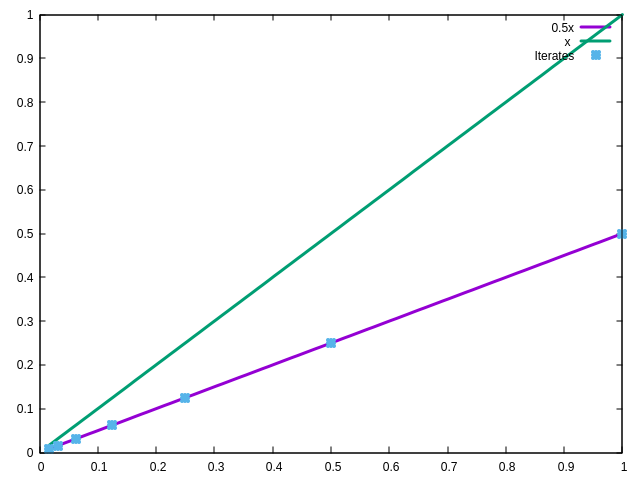
\includegraphics[width=0.5\textwidth]{banachiter.png}
    \caption{Iterates of the simplest contraction mapping $f(x) = \alpha x$ with $\alpha \leq 1$ (here, $\alpha = 0.5$) at starting point $x_0 = 1$ tend toward the fixed point $f(x) = x$ at $(0, 0)$. Green: the line $f(x) = x$. Blue: the contraction mapping $f(x) = 0.5x$, respecting $d(0.5x, 0.5y) \leq 0.5d(x, y)$ with $d(x, y) = |y - x|$. Points: iterates of $f(x)$ with $x_0 = 1$.}
    \label{fig:contract}
\end{figure}

\begin{thm}[Banach Fixed Point Theorem] \label{thm:banach}
Let $(X, d)$ be a non-empty complete metric space with a contraction mapping $T : X \to X$, then $T$ admits a unique fixed point $x^* \in X$.
Moreover, for any $x_0 \in X$, $T^n(x_0) \to x^*$ as $n\to\infty$
\end{thm}

\begin{proof}
Let $x_0 \in X$ be an arbitrary point and let $\{x_n\}$ be the sequence of iterates such that $\forall n \in \mathcal{N}^+, x_n = T(x_{n-1})$. Then we have
\begin{align*}
    d(x_{n+1}, x_n) &\leq q d(x_n, x_{n-1})\\
    &\leq \ldots\\
    &\leq q^n d(x_1, x_0)
\end{align*}
Let $m, n \in \mathcal{N}^+$ such that $m > n$, then, because $(X, d)$ is a metric space and $T$ is a contraction mapping on $X$,
\begin{align*}
    d(x_m, x_n) &\leq d(x_m, x_{m-1}) + \ldots + d(x_{n+1}, x_n)\\
    &\leq q^{m-1}d(x_1, x_0) + \ldots + q^{n}d(x_1, x_0)\\
    &= q^n d(x_1, x_0) \sum_{k=0}^{m-n-1}q^k\\
    &\leq q^n d(x_1, x_0) \sum_{k=0}^{\infty}q^k\\
    &= \frac{q^n}{1 - q} d(x_1, x_0)
\end{align*}
For some arbitrary $\epsilon$, since $q \in [0, 1)$, there is some $N$ such that
\begin{align*}
    q^N < \frac{\epsilon (1-q)}{d(x_1, x_0)}
\end{align*}
Choosing $m, n > N$ gives
\begin{align*}
    d(x_m, x_n) \leq \frac{q^n}{1 - q} d(x_1, x_0) < \frac{\epsilon (1 - q) d(x_1, x_0)}{(1 - q) d(x_1, x_0)} = \epsilon
\end{align*}
Thus, $\{x_n\}$ is a Cauchy sequence with a limit $x^* \in X$, and it is a fixed point of $T$ because
\begin{align*}
    x^* &= \lim_{n\to\infty} x_n\\
    &= \lim_{n\to\infty} T(x_{n-1})\\
    &= T(\lim_{n\to\infty} x_{n-1}) &\text{Valid because $T$ is continuous}\\
    &= T(x^*)
\end{align*}
Finally, it can be shown by contradiction that the fixed point is unique. Suppose there exists $p_1, p_2 \in X$ such that $p_1 \ne p_2$ and $p_1$ and $p_2$ are fixed points of $T$. Then

\begin{align*}
d(T(p_1), T(p_2)) &= d(p_1, p_2) \leq qd(p_1, p_2)\\
&\iff q = 0 &\text{$q \in [0, 1)$}\\
&\implies d(p_1, p_2) \leq 0 
\end{align*}

Since $d(p_1, p_2) \geq 0$ by definition, this implies $d(p_1, p_2) = 0 \implies p_1 = p_2$, which is a contradiction. \qedhere
\end{proof}


Theorem \ref{thm:banach} tells us that given any point $x_0 \in X$, repeated application of the contraction mapping not only leads to convergence, but also converges to the unique fixed point $x^* \in X$. This will be used in the next section to demonstrate convergence of distributional RL.

\section{Distributional RL}
Distributional Reinforcement Learning was first introduced in \citet{distributional}. We will discuss it in the context of infinite horizon.
First we define The following are all the random variables involved in the MDP:
\begin{enumerate}
    %\item $r_t\sim \text{P}(\cdot|s_t, a_t)$     (non-deterministic reward)
    \item $r_t, s_t \sim \text{P}(\cdot,\cdot \,|s_{t-1}, a_{t-1})$ (non-deterministic reward and transition)
    \item $a_t \sim \pi(\cdot \,|s_{t-1})$ (non-deterministic policy)
\end{enumerate}
Using these variables, we can define what is known as the return:
\begin{defn}[Return]
\label{def:Return}
Let $(s_t,a_t)_{t=1}^\infty$ be the state-action pairs of an infinite horizon MDP with a discount factor $0<\gamma\leq1$.
The \textbf{return} is defined as
\begin{equation}
    \Phi^\pi(s, a)=r_0+\sum_{t=1}^{\infty} \gamma^t r_t \,\,\, \, \, \, \text{with } s_0=s \text{ and } a_0 = a 
\end{equation}
which is a function that takes an initial state and action pair as input and output a random variable on the initial state and action. 
\end{defn}

As return, $\Phi^\pi(s,a)$, is a random variable, it has a law, or a distribution.  
Let $\mathcal{D}$ denote \textbf{the space of all distributions of return}.
We define the value distribution as a mapping from the state-action space to the space of distributions of return below.

\begin{defn}[Value Distribution] \label{def:valueDistribution}
Then we define the value distribution as
$$Z^\pi:\mathcal{S}\times \mathcal{A} \rightarrow \mathcal{D}$$
such that
\begin{equation*}
 \Phi^\pi(s, a) \sim Z^\pi(s, a)
\end{equation*}
 $\mathcal{D}^{|\mathcal{S}|\times|\mathcal{A}|}$. Since $Z^\pi(a, s)$ is a distribution, we can write in the discrete case
$$P(\Phi=\phi)=Z^\pi(a, s)(\phi)$$
\end{defn}


It is important to understand that for given a and s, $\Phi^\pi(s, a)$ is a random variable and $Z^\pi(s, a)$ is the distribution of that random variable.
The return and value distributions are linked to the state-action value function described last lecture via the formula 
\begin{equation}
    Q^\pi(s, a) := \E_{Z^\pi(s, a)}[\Phi(s, a)]
\end{equation}

\begin{figure}[H]
    \centering
    \begin{tikzpicture}
    \draw [<->] (0, 5) -- (0, 0) -- (7, 0);
    \node at (7, -1/2) {$\phi$ (return)};
    \node at (-1, 4) {probability};
    \node[text=blue] at (5, 3) {$Z^\pi(a, s)(\phi)$} ;
    \draw [fill=blue] (1, 0) rectangle (1.5, 1);
    \draw [fill=blue] (1.5, 0) rectangle (2, 2);
    \draw [fill=blue] (2, 0) rectangle (2.5, 2.7);
    \draw [fill=blue] (2.5, 0) rectangle (3, 4);
    \draw [fill=blue] (3, 0) rectangle (3.5, 3.6);
    \draw [fill=blue] (3.5, 0) rectangle (4, 2.5);
    \draw [fill=blue] (4, 0) rectangle (4.5, 1.2);
    \draw [fill=blue] (4.5, 0) rectangle (5, 1);
    \draw [fill=blue] (5, 0) rectangle (5.5, 1.5);
    \draw [fill=blue] (5.5, 0) rectangle (6, 1);
    
    \draw [dotted,line width = 1mm] (3.25, 0) -- (3.25, 5);
    \node at (4, 5) {$Q
    ^\pi(a, s)$};
    \end{tikzpicture}
    \caption{example of distribution $Z^\pi(a,s)(\phi)$}
\end{figure}

But why would we want to use the distribution instead of its expectation. The problem with expectation is that we lose information about the random variables. \\

For example lets take two dice (A, B) and play a game. The user must choose a die and throw it once. If die A lands on an even number, the player gets 1 dollar and he loses 1 otherwise. If die B land on ${1, 2, 3, 4 ,5}$ he gets 20 dollars and loses 100 dollars if it lands on 6. 
Both dice have an expectation of 0,
%, which means that the
%gain would average to the same value if the number of throws went to infinity
%However, there is only on dice toss so 
but the two choices involve different levels of risk as they have different distributions. 
This risk cannot be characterized by simply looking at the expectation because both dice are indistinguishable in the sense of expectation, which does not reflect the other statistics of the distribution (such as variance).\\

Before anything else, we define some algebraic operations between distributions:
\begin{defn}
\label{def:algebraic operations on distributions}
Let $Z_1$, $Z_2$ be two independant univariate distributions and let $\gamma \in \mathbb{R}$ be a constant 
We define:
\begin{enumerate}
    \item $(Z_1+Z_2)(x) := (Z_1 * Z_2)(x)$    ( convolutionnal product)
    \item $(\gamma \, Z_1)(x) := \frac{1}{\gamma}Z_1(\gamma x) $      (contracting the function horizontally)
    \item $(\gamma + Z_1)(x) := Z_1(x - \gamma)$     (horizontal translation)
\end{enumerate}
\end{defn}

Now we turn to policy evaluation using distributional RL. The policy $\pi$ is fixed and we want to find the value distribution $Z^\pi(s, a)$ for a given $(s,a)$ pair. First we define the transition operator:
\begin{defn}[Transition Operator]
\label{def:Transition Operator}
$$P^\pi:\mathcal{D}\rightarrow \mathcal{D}$$
\begin{equation}
    P^\pi Z(s, a) = Z(S', A') 
\end{equation}
where $S'\sim P(.|s, a)$ and $A'\sim \pi(.|S')$. Capital letter are used to emphasize the randomness of the new state and action.
\end{defn} 
The output of this operator can be seen as a mixture distribution with weight $P(S'=s', A'=a'|a, s)$ for the each component distribution $Z^\pi(s', a')$.
In what follows, we assume the randomness in the reward and the transition $P^\pi$ are independent. 
Another operator that we define below is the distributional Bellmann operator:
\begin{defn}[Distributional Bellmann operator]
\label{def:Distributional Bellmann operator}
$$\mathcal{T}^\pi:\mathcal{D}\rightarrow \mathcal{D}$$
\begin{equation}
    \mathcal{T}^\pi Z(s, a) = \text{Distr}(r) + \gamma \mathcal{P}^\pi Z(s, a)
\end{equation}
where $\text{Dist}(r)$ is the distribution of rewards at a given state $s$ and by doing the action $a$.
We could also change the input and output spaces of the operator so it acts on random variables instead of their distributions
\begin{equation}
    \mathcal{T}^\pi \Phi^{\pi'}(s, a) \overset{D}{=} r + \gamma \mathcal{P}^\pi \Phi^{\pi'}(s, a)
\end{equation}
These two definitions are equivalent (in the sense of distribution).
\end{defn}
Here is a graphical explanation of the operator with deterministic reward:
\begin{figure}[H]
\centering
\begin{tikzpicture}
\draw [<->] (0, 2) -- (0, 0) -- (3, 0);
\draw [<->] (5, 2) -- (5, 0) -- (8, 0);
\draw [<->] (10, 2) -- (10, 0) -- (13, 0);

\draw[fill=red] (0.5, 0) rectangle (1, 1/2);
\draw[fill=red] (1, 0) rectangle (1.5, 2/2);
\draw[fill=red] (1.5, 0) rectangle (2, 2.4/2);
\draw[fill=red] (2, 0) rectangle (2.5, 1/2);
\node[text=red] at (1.5, 1.5) {$P^\pi Z_\pi(s, a)$};

\draw[->] (4, 0.5) -- (4.75, 0.5);
\draw[fill=blue] (5.25, 0) rectangle (5.5, 1);
\draw[fill=blue] (5.5, 0) rectangle (5.75, 2);
\draw[fill=blue] (5.75, 0) rectangle (6, 2.4);
\draw[fill=blue] (6, 0) rectangle (6.25, 1);
\node[text=blue] at (7, 1.5) {$\gamma P^\pi Z^\pi(s, a)$};
\draw[<-] (6.7, 0.5) -- (7.4, 0.5);

\draw[fill=violet] (10.25+1.5, 0) rectangle (10.5+1.5, 1);
\draw[fill=violet] (10.5+1.5, 0) rectangle (10.75+1.5, 2);
\draw[fill=violet] (10.75+1.5, 0) rectangle (11+1.5, 2.4);
\draw[fill=violet] (11+1.5, 0) rectangle (11.25+1.5, 1);
\node[text=violet] at (11+1.5, 2.6) {$ r(a, s) + \gamma P^\pi Z^\pi (s, a)$};
\draw[->] (10.5, 0.5) -- (11.5, 0.5);
\end{tikzpicture}
\caption{Illustration of how $\mathcal{T}^\pi$ operates on a distribution}
\end{figure}
The final operation is simply a translation because $r$ is deterministic in that example. In a more general case, the right-most distribution would have been obtained with a convolutional product.
It is important to note that $\mathcal{T}^\pi$ resembles the Bellman equations for expected reward. 
In the spirit of policy evaluation, we want to show that the operator is a contraction mapping with respect to some metric. 
Let's first introduce the Wasserstein metric between distributions.

%Policy iteration algorithm


\begin{defn}
\label{def:wass}
Let $Z_1$ and $Z_2$ be two distributions; i.e. $Z_1,Z_2\in\mathcal{D}$. For $p\geq1$, the $p$-Wassertein metric is defined as
\begin{equation}
    d_p(Z_1,Z_2)=\underset{D \in  \prod (Z_1, Z_2) }{\inf}\E_{(z_1,z_2)\sim D}[||z_1 - z_2||_p^p]^{\frac{1}{p}}
\end{equation} 
where $\prod (Z_1, Z_2)$ is the set of all joint distributions with marginals $Z_1$ and $Z_2$. The metric has the following properties (for $\gamma \in \mathbb{R}$ and $a$, a random variable independent of $z_1$ and $z_2$ that follows distribution $A$):
\begin{enumerate}
    \item $d_p(\gamma Z_1, \gamma Z_2) \leq |\gamma| d_p(Z_1, Z_2)$
    \item $d_p(A+Z_1, A+Z_2) \leq d_p(Z_1, Z_2)$
    \item $d_p(A Z_1, A Z_2) \leq ||a||_p d_p(Z_1, Z_2)$
\end{enumerate}
\end{defn}

Note that the Wasserstein metrics are metrics of distributions, whereas value distributions are mappings (from the space of state-action pairs to the space of distributions), the former are not yet metrics of the latter.
Let $\mathcal{Z}$ denote the \textbf{space of value distributions} (with bounded moments).
Let us define a uniform form of the Wasserstein distance as 
$$\bar{d}_p(Z_1,Z_2) = \sup_{s,a} d_p(Z_1(s,a), Z_2(s,a))$$
for $Z_1,Z_2\in\mathcal{Z}$.
Then we can establish the following result.
\begin{lem}
$\bar{d}_p$ is a metric over value distributions.
\end{lem}
The only nontrivial part to prove is triangle inequality of a metric.
\begin{proof}
For $Y\in\mathcal{Z}$, we have 
\begin{align*}
\bar{d}_p(Z_1,Z_2) &= \sup_{s,a} d_p(Z_1(s,a), Z_2(s,a)) \\
&\leq \sup_{s,a} d_p(Z_1(s,a), Y(s,a))+ d_p(Y(s,a), Z_2(s,a)) \\
&\leq \sup_{s,a} d_p(Z_1(s,a), Y(s,a))+ \sup_{s,a} d_p(Y(s,a), Z_2(s,a)) \\
&= \bar{d}_p(Z_1,Y)+\bar{d}_p(Y,Z_2)
\end{align*}
where the first inequality is because $d_p$ is a metric which admits triangle inequality over the space of distributions.
\end{proof}


Now consider the metric space $(\mathcal{Z}, \bar{d}_p)$. 
Considering the iterative process $Z_{k+1}:=\mathcal{T}^\pi Z_k$ with some initial value distirbution $Z_0\in\mathcal{Z}$, we now show that ``distributional'' Bellman operator is a contraction mapping. 
\begin{lem}
$\mathcal{T}^\pi:\mathcal{Z}\rightarrow\mathcal{Z}$ is a $\gamma$-contraction in $\bar{d}_p$.
\end{lem}
\begin{proof}
Let $Z_1,Z_2\in\mathcal{Z}$. 
\begin{align*}
\bar{d}_p(\mathcal{T}^\pi(Z_1),\mathcal{T}^\pi(Z_2)) &= \sup_{s,a} d_p(\mathcal{T}^\pi(Z_1),\mathcal{T}^\pi(Z_2)) \\
&= \sup_{s,a} d_p(Distr(r; s,a) + \gamma P^\pi Z_1(s,a),Distr(r; s,a) + \gamma P^\pi Z_2(s,a)) \\
&\leq \sup_{s,a} \gamma d_p( P^\pi Z_1(s,a),P^\pi Z_2(s,a)) \\
&\leq \sup_{s,a} \gamma \sup_{s',a'} d_p(  Z_1(s',a'), Z_2(s',a')) \\
&= \gamma \bar{d}_p(Z_1, Z_2) 
\end{align*}
where the first two lines are just the definitions of $\bar{d}_p$ and $\mathcal{T}^\pi$; 
the third line is due to the properies of Wasserstein distance (Definition~\ref{def:wass}) and the (conditional) independence of reward and the transition; 
the fourth line is due to taking the sup rather than taking a random next state-action pair. 
\end{proof}

By construction, $Z^\pi$ is a fixed point of the Bellman equation, and by the Banach fixed point theorem, the sequence $(Z_k)_{k\geq1}$ will converge in $\bar{d}_p$ to $Z^\pi$.


\section{Summary}

In this lecture, we saw the infinite horizon variant of RL. We introduced the Banach fixed point theorem, a central theorem to many convergence results in and outside RL algorithms, and used it to demonstrate convergence for distributed RL methods.


%----------------------------------------
\bibliographystyle{abbrvnat}
\bibliography{Refs/notes19b.bib}
%----------------------------------------
\end{document}
